\documentclass[11pt]{article}

%\pagestyle{headings}

\textwidth=440pt
\hoffset=-0.6truein

\usepackage{amsmath}
\usepackage{amsfonts}
\usepackage{amssymb}
\usepackage{authblk}
\usepackage{dsfont}
\usepackage{pifont}
\usepackage{booktabs}
\usepackage{tabularx}
\usepackage{siunitx}
%\usepackage{bbold}
\usepackage{graphicx}
\usepackage{epstopdf}
\usepackage{epsfig}
%\usepackage{bibunits}
%\usepackage{theorem}
%\usepackage[framed]{ntheorem}
\usepackage{framed}
%\usepackage{showlabels}
\usepackage{makeidx}
\usepackage{simplewick}
%\usepackage{tikz-feynman}
\usepackage{hyperref}
\usepackage{placeins}
\usepackage{bbold}
\usepackage[font=small,labelfont=bf]{caption}
%\tikzfeynmanset{compat=1.0.0}
\usepackage{tikz}
\usepackage{braket}
\usetikzlibrary{positioning}% To get more advances positioning options
\usetikzlibrary{arrows}
\usetikzlibrary{colorbrewer}

% barn deprecated by siunitx
\DeclareSIUnit{\barn}{b}

% General global commands
%\newcommand{\cov}{C}
\newcommand{\posterior}[1]{\tilde{#1}}
\newcommand{\real}{\mathbb{R}}
\newcommand{\textin}{\text{in}} 

% General inverse Problems
% map operators
\newcommand{\fwdmapop}{G}
\newcommand{\obsop}{O}
\newcommand{\fwdobsop}{\mathcal{\fwdmapop}}
% model space
\newcommand{\nmodel}{N_{\rm model}}
\newcommand{\modelspace}{X}
\newcommand{\modelvec}{u}
\newcommand{\modelpriorcent}{\modelvec_0}
\newcommand{\modelpriorcov}{\cov_X}
\newcommand{\modelpostcent}{\posterior{\modelvec}}
\newcommand{\modelpostcov}{\posterior{\cov}_X}
% observable space
\newcommand{\ndata}{N_{\rm data}}
\newcommand{\obs}{y}
\newcommand{\obspriorcent}{\obs_0}
\newcommand{\obspriorcov}{\cov_{Y}}
\newcommand{\obsnoise}{\eta}
\newcommand{\obspostcent}{\posterior{\obs}}
\newcommand{\obspostcov}{\posterior{\cov}_Y}
% linear map
\newcommand{\linmap}{\fwdobsop}
\newcommand{\vander}{\mathcal{X}}
\newcommand{\nlaw}{N_{\rm law}}

% NNPDF data/model
\newcommand{\law}{f}
\newcommand{\pseudodat}{\mu}
\newcommand{\noise}{\epsilon}
\newcommand{\repind}{(k)}
\newcommand{\modelvecrep}{\modelvec_*^{\repind}}
% likelihood
\newcommand{\likelihood}{\mathcal{L}}
\newcommand{\repchis}{{\chi^2}^{\repind}}

% closure fitting
\newcommand{\lawmodel}{w}
\newcommand{\utrue}{u_\mathrm{true}}
\newcommand{\uest}{u_\mathrm{est}}

% closure estimators
\newcommand{\testset}[1]{ {{#1}^{\prime}} }
\newcommand{\emodel}[1]{ \mathbf{E}_{\{ \modelvec_* \}} \left[ #1 \right] }
\newcommand{\eout}{\mathcal{E}^{\rm out}}

\newcommand{\nfits}{N_{\rm fits}}
\newcommand{\nreps}{N_{\rm rep}}

\newcommand{\bias}{{\rm bias}}
\newcommand{\var}{{\rm variance}}
\newcommand{\covrep}{\testset{\cov}^{(\rm replica)}}
\newcommand{\covcent}{\testset{\cov}^{(\rm central)}}
\newcommand{\biasvarratio}{\mathcal{R}_{bv}}

% quantile estimators
\newcommand{\xisigdat}[1]{\xi^{(\rm data)}_{#1 \testset{\sigma}}}
\newcommand{\xisigdati}[1]{\xi^{(\rm data)}_{#1 {\testset{\sigma}_i}}}
\newcommand{\modelstd}{\hat{\sigma}}
\newcommand{\erf}{{\rm erf}}

% abbreviations
\newcommand{\ie}{{\it i.e.}}
\newcommand{\eg}{{\it e.g.}}
\newcommand{\viz}{{\it viz.}}

% delta chi2 appendix
\newcommand{\ein}{\mathcal{E}^{\rm in}}
\newcommand{\deltachi}{\Delta_{\chi^2}}
\newcommand{\noisecross}{{\rm noise \, cross \, term}}

% -------------------%
% deprecated commands
% -------------------%
\newcommand{\vv}[1]{\mathbf{#1}}

\newcommand{\vecdiffreptwo}{\left( \vv{\model}^{\repind} - \vv{\levtwo}^{\repind}  \right)}
\newcommand{\vecdiffcentone}{\left( \erep{\vv{\model}} - \vv{\levone} \right)}

\newcommand{\coveig}{\sigma^{2}}
\newcommand{\diag}[1]{\hat{#1}}

\newcommand{\levelonediff}{\Delta}
\newcommand{\underlyingdiff}{u}
\newcommand{\repdiff}{v}

\newcommand{\shiftcross}{{\rm shift \, cross \, term}}
\newcommand{\deltaeps}{\Delta_{\epsilon}}
\newcommand{\kldiv}{D_{KL}}

\newcommand{\diffreptwo}{\left( \model^{\repind} - \levtwo^{\repind} \right)}
\newcommand{\diffcentone}{\left( \erep{\model} - \levone \right)}
\newcommand{\diffcentunder}{\left( \erep{\model} - \law \right)}
\newcommand{\diffcentrep}{\left( \erep{\model} - \model^{\repind}\right)}

\newcommand{\invcov}[1]{\cov^{-1}_{#1}}
\newcommand{\erep}[1]{\mathbf{E}_{\noise}\left[ #1 \right]}
\newcommand{\eshift}[1]{\mathbf{E}_{\shift}\left[ #1 \right]}

\newcommand{\model}{\fwdobsop}
\newcommand{\shift}{\obsnoise}
\newcommand{\invcovprime}{C_D^{\prime -1}}
\newcommand{\levone}{z}
\newcommand{\levtwo}{y}

\newcommand{\npoints}{N_{\rm points}}
\newcommand{\nfit}{\texttt{n3fit}}

\newcommand{\ndat}{N_{\mathrm{dat}}}
\newcommand{\ngrid}{N_{\mathrm{grid}}}
\newcommand{\nflav}{N_{f}}
\newcommand{\NThetaPar}{N_{\Theta\parallel}}
\newcommand{\NThetaPerp}{N_{\Theta\perp}}   
%\newcommand{\nmodel}{N_{\mathrm{model}}}
\newcommand{\cov}{\mathrm{Cov}}
\newcommand{\FKtab}{(\mathrm{FK})}
\newcommand{\FKtabT}{(\mathrm{FK})^T}
\newcommand{\GP}{\mathcal{GP}}
\newcommand{\lat}{{\mathrm{lat}}}
\newcommand{\lin}{{\mathrm{lin}}}
\newcommand{\PDF}{\textrm{PDF}}
\newcommand{\B}{\mathcal{B}} % Basis
\newcommand{\RPDF}{\mathbb{R}^{\PDF}}
\newcommand{\RRPDF}{\mathbb{R}^{\PDF \times \PDF}}
\newcommand{\ddt}{\frac{d}{dt}}
\newcommand{\fin}{f^{\rm in}}

% Matrix
\newcommand{\bpmat}{\begin{pmatrix}}
\newcommand{\epmat}{\end{pmatrix}}

\graphicspath{{./figs/}}

\newcommand{\ldd}[1]{\textcolor{red}{\textbf{Luigi: #1}}}
\newcommand{\ac}[1]{\textcolor{red}{\textbf{Amedeo: #1}}}

\title{Parton Distributions from Neural Networks: Analytical Results}
\author{Amedeo Chiefa}
\author{Luigi Del Debbio}
\author{Richard Kenway}
\affil{Higgs Centre for Theoretical Physics, School of Physics and Astronomy,
Peter~Guthrie~Tait~Road, Edinburgh EH9 3 FD, United Kingdom.}

\date{\today}
\makeindex

\begin{document}

\maketitle

\begin{abstract}
    The determination of Parton Distribution Functions (PDFs) from experimental data
    is a central ingredient in the theoretical prediction of experimental results
    at hadronic colliders. As the LHC is now producing high-precision results, a robust
    determination of PDFs and their associated errors have become increasingly important.
    The NNPDF Colalaboration has pioneered the use of Machine Learning for the determination
    of PDFs. In this paper, we develop a theoretical formalism to analyse the training of
    Neural Networks in the context of PDF determinations.
\end{abstract}

\section{Introduction}
\label{sec:intro}

A first paragraph on precision physics at the LHC and the need for robust determinations of PDFs.

The extraction of PDFs from experimental data is a classic example of an inverse problem,
namely the reconstruction of a function $f(x)$ from a finite set of data points
$Y_I$, where the index $I=1, \ldots, \ndat$.~\footnote{When omitting the data index $I$, we will always
assume $Y \in \mathbb{R}^{\ndat}$.} In particular, for this study, we will focus
on DIS data, which depend
linearly on the function $f(x)$. The theoretical prediction for the data point $Y_I$ is denoted
\begin{equation}
    \label{eq:TheoryPred}
    T_I[f] = \int dx\, C_{Ii}(x) f_{i}(x)\, ,
\end{equation}
where $C_{Ii}(x)$ is a coefficient function, $i$ labels the parton flavor, and $f_i(x)$
is the PDF (or set of PDFs) that we want to determine.

Trying to determine a function $f$ in an infinite dimensional space of solutions with a finite
set of data leads to an ill-defined problem, whose solution will depend on assumptions made.
In particular, the choice of a parametrization for $f$ leads to a bias in the space
of solutions that can be obtained. Together with the fit methodology, the parametrization also
determines the propagation of the error on the data to the error on the fitted solution. Understanding
the bias and the variance of the fitted PDF is therefore a major challenge for precision physics.

Following the ideas highlighted in Refs.~\cite{DelDebbio:2021whr,Candido:2024hjt}, we find it
useful to introduce a Bayesian
framework for this analysis. The function $f$ is promoted to a stochastic process; for any grid
of points $x_{\alpha}$, $\alpha=1, \ldots, \ngrid$, the vector $f_{\alpha}=f(x_{\alpha})$ is a
vector of $\ngrid$ stochastic variables, for which we introduce a prior distribution $p(f)$.~\footnote{Following
the same convention used for the data, when omitting the grid index $\alpha$, we will always refer to a
vector $f \in \mathbb{R}^{\ngrid}$.}

Any fitting procedure is interpreted as a recipe that yields the posterior distribution
$\tilde{p}(f)$.

In this study, probability distributions are represented by ensembles of i.i.d. replicas.
So, for instance, the prior distribution $p(f)$ is described by an ensemble
\begin{equation}
    \label{eq:RepDef}
    \left\{f^{(k)} \in \mathbb{R}^{\ngrid}; k=1, \ldots, \nreps\right\}\, ,
\end{equation}
drawn from the distribution $p$, so that
\begin{equation}
    \label{eq:ReplicaEnsemble}
    \mathbb{E}_{p}[O(f)] = \frac{1}{\nreps} \sum_{k=1}^{\nreps} O(f^{(k)})\, ,
\end{equation}
for any observable $O$ that is built from the PDFs.

The prior distribution $p(f)$ is defined by initializing a set of replicas using a Glorot-Normal initializer.
The result of this initialization is discussed below in Sec.~\ref{sec:Init}.
For each replica, a new set of data $Y^{(k)}$ is generated from an $\ndat$ dimensional Gaussian distribution
centred at the experimental central value $Y$, with the covariance given by the experimental covariance
matrix $C_Y$,
\begin{equation}
    \label{eq:ExpReplicaDistr}
    Y^{(k)} \sim \mathcal{N}\left(Y, C_Y\right)\, .
\end{equation}
Each replica is $f^{(k)}$ trained on its corresponding data set $Y^{(k)}$. We denote the replicas at training time $t$,
$f^{(k)}_{t} \in \mathbb{R}^\ngrid$. Stopping the training at time $\bar{t}$, the posterior probability
distribution is represented by the set of replicas $\left\{f^{(k)}_{\bar{t}}\right\}$, so that
\begin{equation}
    \label{eq:PostEnsemble}
    \mathbb{E}_{\tilde{p}}[O(f)] = \frac{1}{\nreps} \sum_{k=1}^{\nreps}
        O\left(f^{(k)}_{\bar{t}}\right)\, .
\end{equation}
All knowledge about the solution of the inverse problem, $f$, is encoded in the posterior
$\tilde{p}$ and is expressed as expectation values of observables $O$ using
Eq.~\eqref{eq:PostEnsemble}.

\section{Neural Networks at Initialization}
\label{sec:Init}

As detailed in Ref.~\cite{NNPDF:2021njg}, the NNs used for the NNPDF fit have a 2-25-20-8 architecture,
a $\tanh$ activation function
and are initialized using a Glorot normal distribution~\cite{glorot2010understanding}. The preactivation
function of a neuron is denoted as $\phi^{(\ell)}_{i,\alpha} = \phi^{(\ell)}_i(x_\alpha)$, where $\ell$
denotes the layer of the neuron, $i$ identifies the neuron within the layer~\footnote{We will refer
to $i$ as the {\em neuron}\ index.}, and $x_{\alpha}$ is a point in the interval $[0,1]$.
A grid of $\ngrid=50$ points is used to compute observables in the NNPDF formalism and we will focus
on those values of $x_\alpha$ here. For completeness, we list the values of $x_\alpha$ in
Tab.~\ref{tab:Xvals}.

\begin{table}[ht]
    \centering
    \begin{tabular}{|c|c|c|c|c|c|c|c|c|c|}
    \hline
    $\alpha$ & $x_\alpha$ & $\alpha$ & $x_\alpha$ & $\alpha$ & $x_\alpha$ & $\alpha$ & $x_\alpha$ & $\alpha$ & $x_\alpha$ \\
    \hline
    $1$  & $2.00 \times 10^{-7}$ & $11$ & $1.29 \times 10^{-5}$ & $21$ & $8.31 \times 10^{-4}$ & $31$ & $0.0434$ & $41$ & $0.422$ \\
    $2$  & $3.03 \times 10^{-7}$ & $12$ & $1.96 \times 10^{-5}$ & $22$ & $1.26 \times 10^{-3}$ & $32$ & $0.0605$ & $42$ & $0.480$ \\
    $3$  & $4.60 \times 10^{-7}$ & $13$ & $2.97 \times 10^{-5}$ & $23$ & $1.90 \times 10^{-3}$ & $33$ & $0.0823$ & $43$ & $0.540$ \\
    $4$  & $6.98 \times 10^{-7}$ & $14$ & $4.51 \times 10^{-5}$ & $24$ & $2.87 \times 10^{-3}$ & $34$ & $0.109$ & $44$ & $0.601$ \\
    $5$  & $1.06 \times 10^{-6}$ & $15$ & $6.84 \times 10^{-5}$ & $25$ & $4.33 \times 10^{-3}$ & $35$ & $0.141$ & $45$ & $0.665$ \\
    $6$  & $1.61 \times 10^{-6}$ & $16$ & $1.04 \times 10^{-4}$ & $26$ & $6.50 \times 10^{-3}$ & $36$ & $0.178$ & $46$ & $0.730$ \\
    $7$  & $2.44 \times 10^{-6}$ & $17$ & $1.57 \times 10^{-4}$ & $27$ & $9.70 \times 10^{-3}$ & $37$ & $0.220$ & $47$ & $0.796$ \\
    $8$  & $3.70 \times 10^{-6}$ & $18$ & $2.39 \times 10^{-4}$ & $28$ & $0.0144$ & $38$ & $0.265$ & $48$ & $0.863$ \\
    $9$  & $5.61 \times 10^{-6}$ & $19$ & $3.62 \times 10^{-4}$ & $29$ & $0.0211$ & $39$ & $0.314$ & $49$ & $0.931$ \\
    $10$ & $8.52 \times 10^{-6}$ & $20$ & $5.49 \times 10^{-4}$ & $30$ & $0.0305$ & $40$ & $0.367$ & $50$ & $1.00$ \\
    \hline
\end{tabular}

    \caption{Values of $x_\alpha$ used in the NNPDF grids for the computation of
    observables. The points are equally spaced on a logarithmic scale
    for $\alpha = 1, \ldots, XXX$, and linearly spacing for $\alpha > XXX$.
    \ac{Maybe we need to rethink the layout of this table...}
    \label{tab:Xvals}}
\end{table}

The output of the neuron identified by the pair $(\ell,i)$ is
$\rho^{(\ell)}_{i,\alpha} = \tanh\left(\phi^{(\ell)}_{i,\alpha}\right)$.
The parameters of the NN are the weights $w^{(\ell)_{ij}}$ and the biases $b^{(\ell)}_i$, which are
collectively denoted as $\theta_\mu$, where $\mu = 1, \ldots, P$ and the total number of parameters
is
\begin{equation}
    \label{eq:TotPar}
    P = \sum_{\ell=1}^{L} \left(n_{\ell} n_{\ell-1} + n_\ell\right)\, .
\end{equation}
The PDFs in the
so-called evolution basis are parametrized by the preactivation functions of the output layer $L$,
$f_i(x_\alpha)=A_i \phi^{(L)}_{i,\alpha}$, where $i=1, \ldots, 8$ labels the flavors.
~\footnote{For simplicity, we ignore the preprocessing function $x^{-\alpha_i} (1-x)^{\beta_i}$ that
is currently used in the NNPDF fits. While the preprocessing may be useful in speeding the training
it does not affect the current discussion.}
The input layer is identified by $\ell=0$ and the activation
function for that specific layer is the identity, so that
\begin{equation}
    \label{eq:InitLayerPhi}
    \rho^{(0)}_{i,\alpha} = \phi^{(0)}_{i,\alpha} = x_{i,\alpha} =
    \begin{cases}
        x_\alpha\, , \quad &\text{for}\ i=1\, ;\\
        \log\left(x_\alpha\right)\, , \quad &\text{for}\ i=2\, .
    \end{cases}
\end{equation}
In the following we refer to the preactivation functions as {\em fields}.

The Glorot normal initialiser draws each weight and bias of the NN from independent Gaussian
distributions, denoted $p_w$ and $p_b$ respectively, centred at zero and with variances
rescaled by the number of nodes in adjacent layers,
\begin{equation}
    \label{eq:RescaledGlorotVariances}
    \frac{C^{(\ell)}_{w}}{\sqrt{n_{\ell-1} + n_{\ell}}}\, ,
    \quad \frac{C^{(\ell)}_{b}}{\sqrt{n_{\ell-1} + n_{\ell}}}\, .
\end{equation}
The probability distribution of the NN parameters induces a probability distribution for the
preactivations,
\begin{align}
    \label{eq:PreactAtInit}
    p\left(\phi^{(\ell)}\right)
      &= \int \mathcal{D}w\, p_w(w)\,
        \mathcal{D}b\, p_b(b)\, \prod_{i,\alpha}
        \delta\left(
          \phi^{(\ell)}_{i\alpha} - \sum_{j} w^{(\ell)}_{ij}
          \rho\left(\phi^{(\ell-1)}_{j\alpha}\right)
          - b^{(\ell)}_i
          \right)\, .
\end{align}
Note that, here and in what follows, $p(\phi^{(\ell)})$ denotes the joint probability for all the components
of $\phi^{(\ell)}$,
\begin{align}
    \label{eq:ExplIndices}
    p\left(\phi^{(\ell)}\right) = p\left(\phi^{(\ell)}_{1,\alpha_1}, \phi^{(\ell)}_{2,\alpha_1}, \ldots,
        \phi^{(\ell)}-{n_\ell,\alpha_1}, \ldots,
        \phi^{(\ell)}_{n_\ell,\ngrid}\right)\, .
\end{align}
This duality between parameter-space and function-space provides a powerful framework to study
the behaviour of an ensemble of NNs, and in particular the symmetry properties of the distribution
$p(\phi^{(\ell)})$, see \eg~\cite{Maiti:2021fpy}. Working in parameter space, \ie\ computing the
expectation values of correlators of fields as integrals over the NN parameter, one can readily
show that
\begin{align}
    \label{eq:NeurRotInv}
    \mathbb{E}\left[
        R_{i_1j_1} \phi^{(n_\ell)}_{j_1 \alpha_1} \ldots
        R_{i_nj_n} \phi^{(n_\ell)}_{j_n \alpha_n}
    \right] =
    \mathbb{E}\left[
        \phi^{(n_\ell)}_{i_1 \alpha_1} \ldots
        \phi^{(n_\ell)}_{i_n \alpha_n}
    \right]\, ,
\end{align}
where $R$ is an orthogonal matrix in $\text{SO}(n_{\ell})$. Eq.\eqref{eq:NeurRotInv} implies
that the probability distribution in Eq.~\eqref{eq:PreactAtInit} is also invariant under rotations,
and therefore it can only be a function of $\text{SO}(n_{\ell})$ invariants. Therefore
\begin{align}
    \label{eq:PriorAction}
    p\left(\phi^{(n_\ell)}\right) =
        \frac{1}{Z^{(\ell)}} \exp\left(-S\left[\phi^{(\ell)}_{\alpha_1}
            \cdot \phi^{(\ell)}_{\alpha_2}\right]\right)\, ,
\end{align}
where
\begin{align}
    \label{eq:PhiInvariant}
    \phi^{(\ell)}_{\alpha_1}
            \cdot \phi^{(\ell)}_{\alpha_2} =
    \sum_{i=1}^{n_\ell} \phi^{(\ell)}_{i \alpha_1} \phi^{(\ell)}_{i \alpha_2}\, .
\end{align}
The action can be expanded in powers of the invariant bilinear,
\begin{align}
    \label{eq:ExpandAction}
    S\left[\phi^{(\ell)}_{\alpha_1}
            \cdot \phi^{(\ell)}_{\alpha_2}\right] =
        \frac12 \gamma^{(\ell)}_{\alpha_1\alpha_2}
            \phi^{(\ell)}_{\alpha_1} \cdot \phi^{(\ell)}_{\alpha_2} +
            \frac{1}{8 n_{\ell-1}} \gamma^{(\ell)}_{\alpha_1\alpha_2,\alpha_3\alpha_4}
            \phi^{(\ell)}_{\alpha_1} \cdot \phi^{(\ell)}_{\alpha_2} \,
            \phi^{(\ell)}_{\alpha_3} \cdot \phi^{(\ell)}_{\alpha_4} + O(1/n_{\ell-1}^2)\, ,
\end{align}
so that the probability distribution is fully determined by the couplings $\gamma^{(\ell)}$. In
Eq.~\eqref{eq:ExpandAction}, we have factored out inverse powers of $n_\ell$ for each coupling.
With this convention, and with the scaling of the parameters variances in
Eq.~\eqref{eq:RescaledGlorotVariances}, the couplings in the action are all $O(1)$
in the limit where $n_\ell\to\infty$.
As a consequence, the probability distribution at initialization is a multidimensional Gaussian at
leading order in $1/n_\ell$, with quartic corrections that are $O(1/n_\ell)$, while higher powers
of the invariant bilinear are suppressed by higher powers of the width of the layer. This power counting
defines an effective field theory, where deviations from Gaussianity can be computed in perturbation
theory to any given order in $1/n_\ell$, see \eg\ Ref.~\cite{Roberts:2021fes} for a detailed
presentation of these ideas. While the actual calculations become rapidly cumbersome, the
conceptual framework is straightforward.

At leading order, the second and fourth cumulant are respectively
\begin{align}
    &\langle \phi^{(\ell)}_{i_1,\alpha_1} \phi^{(\ell)}_{i_2,\alpha_2}\rangle
      = \delta_{i_1 i_2} K^{(\ell)}_{\alpha_1\alpha_2} + O(1/n_{\ell-1})\, , \\
    &\langle \phi^{(\ell)}_{i_1,\alpha_1} \phi^{(\ell)}_{i_2,\alpha_2}
      \phi^{(\ell)}_{i_3,\alpha_3} \phi^{(\ell)}_{i_4,\alpha_4}\rangle_c
      = O(1/n_{\ell-1})\, ,
\end{align}
where
\begin{equation}
    \label{eq:DefineKmat}
    K^{(\ell)}_{\alpha_1\alpha_2} = \left(\gamma^{(\ell)}\right)^{-1}_{\alpha_1\alpha_2}\, .
\end{equation}
The ``evolution'' of the couplings as we go deep in the NN, \ie\ the dependence of the couplings on
$\ell$, is governed by Renormalization Group (RG) equations, which preserve the power counting in
powers of $1/n_{\ell}$. At leading order,
\begin{align}
    K^{(\ell+1)}_{\alpha_1\alpha_2} &=
      \left.
      C_b^{(\ell+1)} + C_w^{(\ell+1)} \frac{1}{n_\ell}
      \langle \vec{\rho}^{\,(\ell)}_{\alpha_1} \cdot
      \vec{\rho}^{\,(\ell)}_{\alpha_2} \rangle
      \right|_{O(1)} \\
      \label{eq:RecursionForK}
      &= C_b^{(\ell+1)} + C_w^{(\ell+1)} \frac{1}{n_\ell}
      \langle \vec{\rho}^{\,(\ell)}_{\alpha_1} \cdot
      \vec{\rho}^{\,(\ell)}_{\alpha_2} \rangle_{K^{(\ell)}}\, ,
\end{align}
where
\begin{align*}
    \frac{1}{n_\ell}
      \langle \vec{\rho}^{\,(\ell)}_{\alpha_1} \cdot
      \vec{\rho}^{\,(\ell)}_{\alpha_2} \rangle_{K^{(\ell)}} =
    \int \prod_{\alpha}d\phi_\alpha\,
      \frac{e^{-\frac12 \left(K^{(\ell)}\right)^{-1}_{\beta_1\beta_2}
        \phi_{\beta_1} \phi_{\beta_2}}}
        {\left|2\pi K^{(\ell)}\right|^{1/2}}\,
        \rho(\phi_{\alpha_1}) \rho(\phi_{\alpha_2})\, .
\end{align*}
Eq.~\eqref{eq:RecursionForK} can be solved for the NNPDF architecture leading to the
covariance matrices for the output of the NNs displayed in
Figs.~\ref{Fig:KRecursionOne} and~\ref{Fig:KRecursionTwo}.
\begin{figure}[t!]
    \centering
    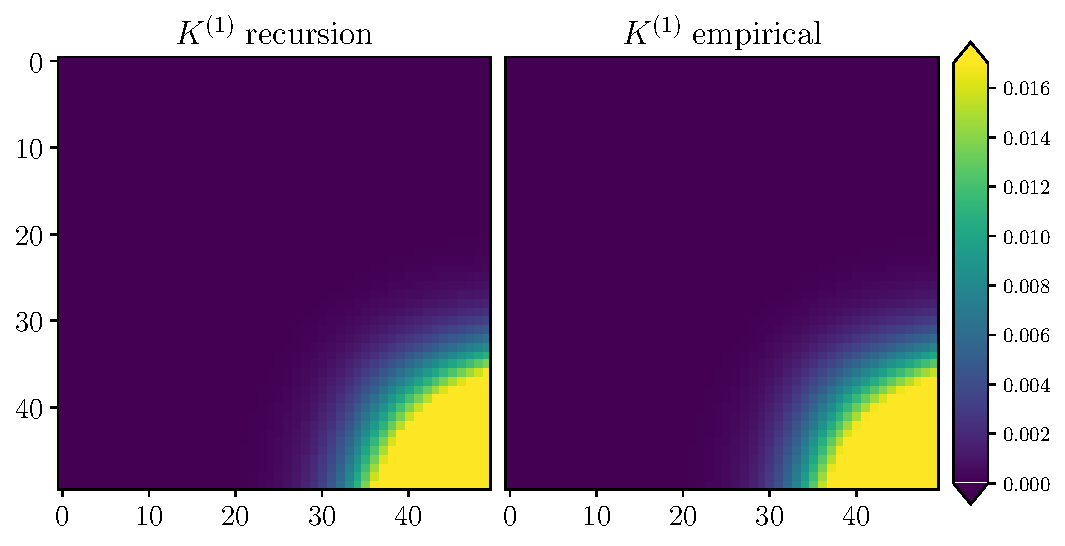
\includegraphics[scale=0.4]{figs/K1_correlations.pdf}
    \caption{The empirical (left) and analytical (right) covariance matrices $K^{(1)}$ of the first layer
    of the NNPDF architecture. The covariance in the left panel is computed ``bootstrapping'' over an
    ensemble of 100 replicas, initialised using the Glorot normal distribution. The covariance in the right
    panel is obtained by solving Eq.~\eqref{eq:RecursionForK} numerically.
    \label{Fig:KRecursionOne}
    }
\end{figure}

\begin{figure}[t!]
    \centering
    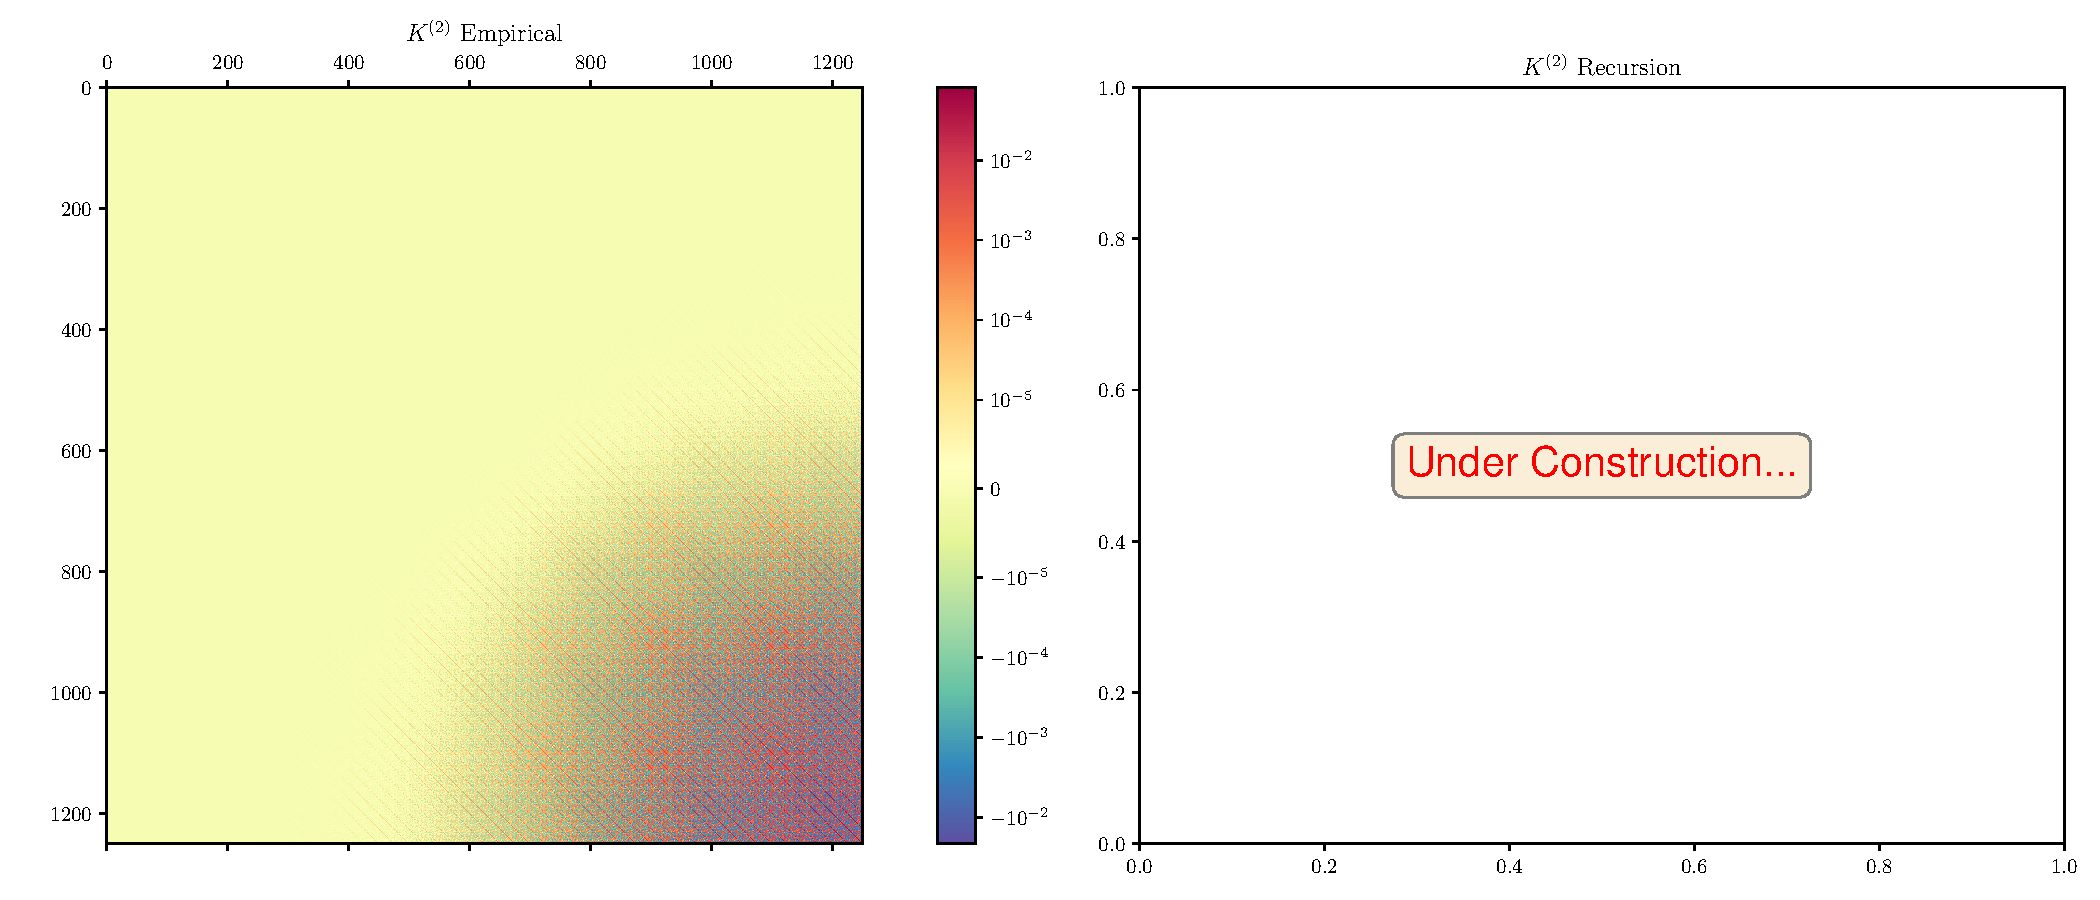
\includegraphics[scale=0.4]{figs/K2_correlations.pdf}
    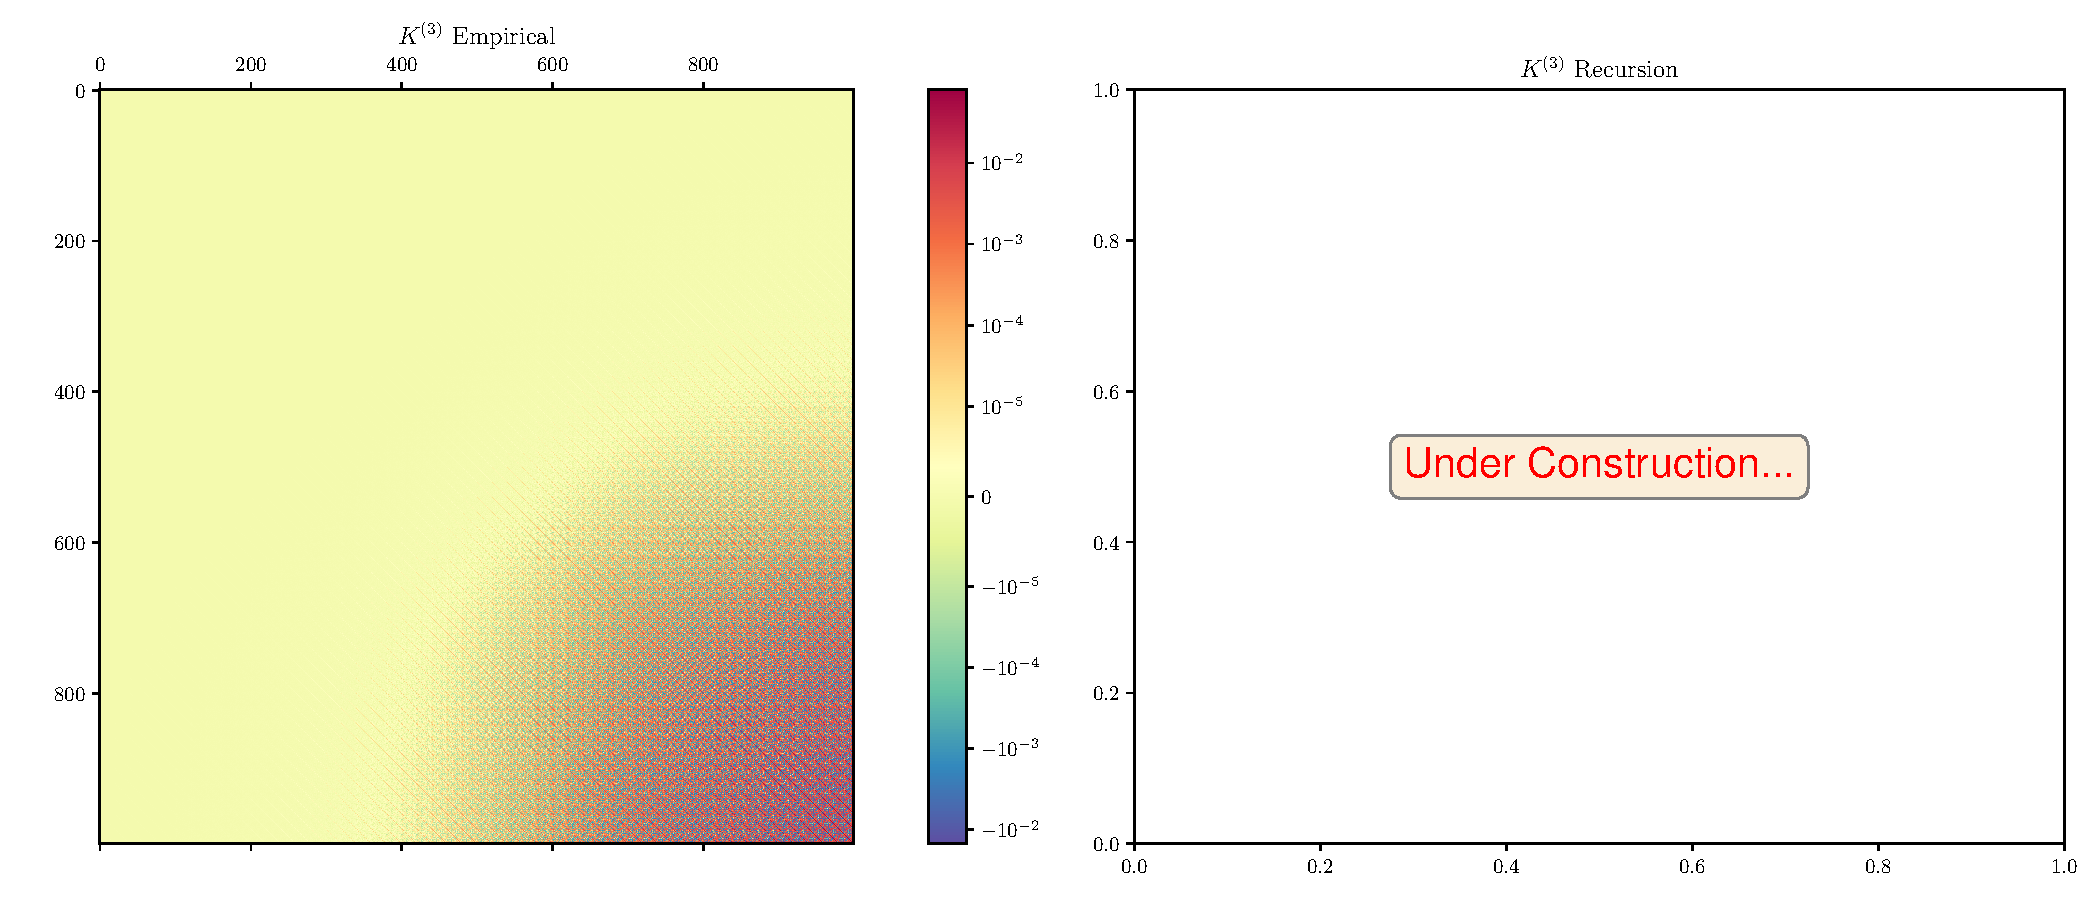
\includegraphics[scale=0.4]{figs/K3_correlations.pdf}
    \caption{Same as Fig.~\ref{Fig:KRecursionOne}, but for the second (top) and third (bottom) layers of the
    NNPDF architecture.
    \ac{Here the four indices of the covariance $K_{i_1i_2, \alpha_1\alpha_2}$ are flattened into
    two indices for the sake of graphical representation. Maybe we should group the labels into groups of
    $N_{\rm grid}$ ticks on the axes.}
    \label{Fig:KRecursionTwo}
    }
\end{figure}

As a consequence of the symmetry of the probability distribution, the mean value of the fields at
initialization needs to vanish, while their variance at each point $x_\alpha$ is given by the
diagonal matrix elements of $K^{(\ell)}$. The central value and the variance of the
parametrized singlet ($\Sigma$) and gluon ($g$) at initialization are shown in
Fig.~\ref{fig:SingletGluonInit} for an ensemble of $\nreps=100$. The central value is computed as
discussed above in Eq.~\eqref{eq:ReplicaEnsemble},
\begin{align}
    \label{eq:MeanValAtInit}
    \bar{f}_{i\alpha} = \bar{f}_{i}(x_\alpha) = \frac{1}{\nreps} \sum_{k=1}^{\nreps} f^{(k)}_i(x_\alpha)\, ,
\end{align}
and the variance $\sigma^2_{i\alpha}$ is computed using the same formula with
\begin{align}
    \label{eq:VarAtInit}
    O(f) = \frac{\nreps}{\nreps-1} \left(f_i(x_\alpha) - \bar{f}_{i}(x_\alpha)\right)^2\, .
\end{align}

\begin{figure}[!ht]
    \begin{center}
        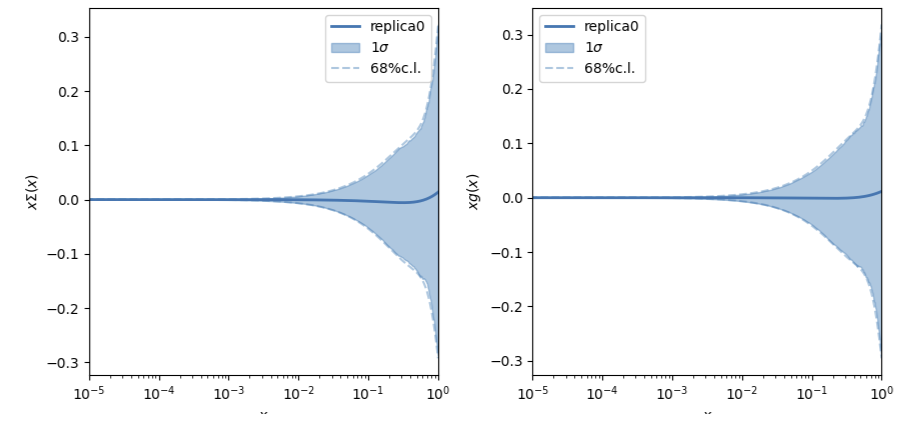
\includegraphics[scale=0.4]{plots/NNPDFAtInit.png}
    \end{center}
    \caption{Parametrized singlet (left) and gluon (right) at initialization. The line labeled
    as Replica0 is the average of the functions over the ensemble of replicas. The blue $1\sigma$ band
    shows the variance of the ensemble of replicas, while the dotted line is the 68\% CL.
    The agreement between these two quantities is a confirmation of the Gaussianity of the
    distribution of replicas.
    \label{fig:SingletGluonInit}
    }
\end{figure}

\paragraph{Dependence on the architecture.}
Having analytical expressions for the variance at initialization allows us to investigate the
impact of the NN architecture on the prior that is imposed on the PDFs. Iterating
Eq.~\eqref{eq:RecursionForK} yields the covariance at initialization for various depths.
Do we get something interesting? worth mentioning?

We should also look at the recursion relations with other activations. Again, check whether we
get something interesting...


\section{Training}
\label{sec:Training}

\subsection{Gradient Flow}
\label{sec:GradFlow}

The parameter-space/function-space duality described in Sec.~\ref{sec:Init} yields intersting insight
on the training process. Our main concern in this paper is understanding the dynamics driving the
training process, therefore we work in a simplified setting where we consider standard gradient descent
and data that depend linearly on the unknwon PDFs, as shown in Eq.~\eqref{eq:TheoryPred}. The generalization
to other minimizers and non-linear data is left to future investigations, but is expected to yield
qualitatively similar results. The results
in this subsection apply to any generic parametrization of the unknown function, they are {\em not}\
specific to the case of using NN for the parametrization.

Gradient descent is described as a continuous flow of the parameters $\theta$ in training time $t$
along the negative gradient of the loss function $\mathcal{L}$. The parameters and the fields during
training are labelled by adding an index $t$, so that \eg\ $\theta_{t,\mu}$ identifies the parameter
$\theta_\mu$ at time $t$.
The gradient flow is given by
\begin{align}
    \label{eq:GradientFlowDef}
    \ddt &\theta_{t,\mu} = -\nabla_\mu \mathcal{L}_t\, .
\end{align}
We focus here on quadratic loss functions that are obtained as the negative logarithm of Gaussian
data distributions around their theoretical predictions,
\begin{align}
    \label{eq:QuadLoss}
    \mathcal{L}_t = \frac12 \left(Y - T[f_t]\right)^T C_Y^{-1} \left(Y - T[f_t]\right)\, ,
\end{align}
where $C_Y$ is the covariance of the data, which includes statistical and systematic errors given by
the experiments and also any theoretical error, like \eg\ missing higher orders in the theoretical
predictions. Indices that are summed over are suppressed to improve the clarity of the equations.
Note that the loss function at training time $t$ is computed using the theoretical prediction $T[f_t]$,
\ie\ the result of Eq.~\eqref{eq:TheoryPred} computed using the fields at training time $t$. For a quadratic
loss, the gradient is
\begin{align}
    \nabla_\mu \mathcal{L}_t = - \left(\nabla_\mu f_t\right)^T \left(\frac{\partial T}{\partial f}\right)_t
      C_Y^{-1} \epsilon_t\, ,
\end{align}
where, writing explicitly the data index,
\begin{align}
    \label{eq:EpsDef}
    \epsilon_{t,I} = Y_I - T_I[f_t]\, , \quad I=1, \ldots, \ndat\, .
\end{align}
For the specific case of a quadratic loss function, the gradient is proportional to $\epsilon_t$, which
is the difference between the theoretical prediction and the data at training time $t$. If at some point
during the training the theoretical predictions reproduce all the data, the training process ends.
A further simplification is obtained in the case of data that depend linearly on the unknown function $f$.
In the specific case of NNPDF fits, the integrals in Eq.~\eqref{eq:TheoryPred} are approximated by
a Riemann sum over the grid of $x$ points,
\begin{align}
    \label{eq:FKTabDef}
    T_I[f] \approx \sum_{\alpha=1}^{\ngrid} \FKtab_{Ii\alpha} f_{i\alpha}\, ,
\end{align}
and hence
\begin{align}
    \label{eq:dTbydf}
    \left(\frac{\partial T_I}{\partial f_{i\alpha}}\right)_t =
        \FKtab_{Ii\alpha}\, ,
\end{align}
and is independent of $t$. The flow of parameters $\theta$ translates into a flow for the fields,
\begin{align}
    \label{eq:NTKFlow}
    \ddt &f_{t,i_1\alpha_1} = (\nabla_\mu f_{t,i_1\alpha_1}) \ddt \theta_\mu =
      \Theta_{t,i_1\alpha_1i_2\alpha_2}
      \FKtabT_{i_2\alpha_2I} \left(C_Y^{-1}\right)_{IJ} \epsilon_{t,J}\, ,
\end{align}
where
\begin{align}
    \label{eq:NTKDef}
    \Theta_{t,i_1\alpha_1i_2\alpha_2} = \sum_\mu
    \nabla_\mu f_{t,i_1\alpha_1} \nabla_\mu f_{t,i_2\alpha_2}\, .
\end{align}
For clarity, we often omit indices and write
\begin{align}
    \left(\frac{\partial T}{\partial f}\right)_t
        &= \FKtab\, , \\
    \Theta_t
        &= \left(\nabla_\mu f_t\right)^T \left(\nabla_\mu f_t\right)\, , \\
    \label{eq:FlowEquationNoIndices}
    \ddt f_t
        &= \Theta_t \FKtabT C_Y^{-1} \epsilon_t\, .
\end{align}
Note that these equations do not refer to a specific parametrization and remain valid when some
explicit functional form is chosen to parametrize the PDFs, as \eg\ in
Refs.~\cite{Bailey:2020ooq,Hou:2019efy}.

\subsection{Lazy Training for the Flow Equation}
\label{sec:Lazy}

The large-$n_{\ell}$ effective theory discussed in Sect.~\ref{sec:Init} also predicts that
the NTK remains constant along training, up to corrections that are $O(1/n_{\ell})$, see
Ref.~\cite{DBLP:journals/corr/abs-1806-07572} and references therein for a derivation of this result.
This regime is sometimes referred to as {\em lazy kernel training}, and allows an analytical
solution of the flow equation.

We start by rewriting Eq.~\eqref{eq:FlowEquationNoIndices} as
\begin{align}
    \label{eq:FlowEqTwo}
    \ddt f_t = -\Theta M f_t + b\, ,
\end{align}
where
\begin{align}
    M &= \FKtabT C_Y^{-1} \FKtab\, , \quad b = \Theta \FKtabT C_Y^{-1} Y\, .
\end{align}
The eigenvectors of $\Theta$,
\begin{align}
    \label{eq:ThetaEigensystem}
    \Theta z^{(k)} = \lambda^{(k)} z^{(k)}\, ,
\end{align}
provide a basis for expanding Eq.~\eqref{eq:FlowEqTwo}. It is necessary at this stage to distinguish
the components of $f_t$ that are in the kernel of $\Theta$ from the ones that are in the orthogonal
complement, hence we introduce the notation
\begin{align}
    &f^\parallel_{t,k} = \left(z^{(k)}, f_t\right)\, , \quad \text{if}\ \lambda_{(k)} = 0\, , \\
    &f^\perp_{t,k} = \frac{1}{\sqrt{\lambda^{(k)}}} \left(z^{(k)}, f_t\right)\, , \quad
        \text{if}\ \lambda^{(k)} \neq 0\, .
\end{align}
One can readily see that the components in the kernel of $\Theta$, $\text{ker}\ \Theta$,
do not evolve during the flow,
\begin{align}
    \label{eq:FlowParallel}
    \ddt f^\parallel_{t,k} = 0
        \quad \Longrightarrow \quad f^\parallel_{t,k} = f^\parallel_{0,k}\, .
\end{align}
The flow equation for the orthogonal components can be written as
\begin{align}
    \label{eq:FlowPerp}
    \ddt f^\perp_{t,k} = - H^\perp_{kk'} f^\perp_{t,k'}
        + B^\perp_{k}\, ,
\end{align}
where the indices on quantities that have a $\perp$ suffix only span the space orthogonal to the kernel
of $\Theta$, while the indices on quantities that have a $\parallel$ suffix span the kernel.
In Eq.~\eqref{eq:FlowPerp}, we introduced
\begin{align}
    H^\perp_{kk'} &= \sqrt{\lambda^{(k)}} \left(z^{(k)}, M z^{(k')}\right) \sqrt{\lambda^{(k')}}\, ,\\
    B^\perp_k &= -\sqrt{\lambda^{(k)}} \left[\left(z^{(k)}, M z^{(k')}\right) f^\parallel_{0,k'}
        - \left(z^{(k)}, \FKtabT C_Y^{-1} Y\right)\right]\, .
\end{align}
We refer to $H^\perp$ as the flow (or training) Hamiltonian; we see explicitly in the definition above that
the flow dynamics is determined by a combination of the architecture of the NN, encoded in the NTK, and the
data, on which $M$ depends. More specifically, the matrix elements of $M$ can be written as
\begin{align}
    \label{eq:MMatElems}
    \left(z^{(k)}, M z^{(k')}\right) = T^{(k)T} C_Y^{-1} T^{(k')}\, ,
\end{align}
where $T^{(k)} = T[z^{(k)}]$ is the vector of theory predictions for the data obtained using $z^{(k)}$ as the
input PDF. Denoting by $d^\perp$ the dimension of the subspace orthogonal to $\text{ker}\ \Theta$, $H^\perp$ is
a $d^\perp\times d^\perp$ symmetric matrix, whose eigenvalues and eigenvectors satisfy
\begin{align}
    H^\perp_{kk'} w^{(i)}_{k'} = h^{(i)} w^{(i)}_{k}\, .
\end{align}
The solution to Eq.~\eqref{eq:FlowPerp} can be written as the sum of the solution of the
homogeneous equation, $\hat{f}^{\perp}_{t,k}$, and a particular solution of the full equation.
The solution of the homogeneous equation is
\begin{align}
    \label{eq:HomoSoln}
    \hat{f}^{\perp}_{t,k} = \sum_{i=1}^{d^\perp} C_i e^{-h^{(i)}t} w^{(i)}_k\, ,
\end{align}
where
% ~\footnote{
%     Note that here the scalar product is computed in the subspace orthogonal to the kernel of $\Theta$,
%     \[
%         \left(w^{(i)}, f^\perp_0\right) = \sum_{k=1}^{d_\perp} w^{(i)}_{k} f^\perp_{0,k}
%     \]
% }
\begin{align}
    \label{eq:InitialCi}
    C_i = \sum_{k=1}^{d_\perp} w^{(i)}_k f^\perp_{0,k}\, ,
        %= \left(w^{(i)}, f^\perp_0\right)\, ,
\end{align}
guarantees that the initial condition $\hat{f}^\perp_{t,k}=f^\perp_{0,k}$ is
satisfied. If we define
\begin{align}
    \label{eq:BiDef}
    B_i = \sum_{k=1}^{d_\perp} w^{(i)}_k B^\perp_{k}\, ,
        %= \left(w^{(i)}, B^\perp\right)\, ,
\end{align}
then
\begin{align}
    \label{eq:PartSol}
    \check{f}^\perp_{t,k} = \sideset{}{'}\sum_{i} \frac{1}{h^{(i)}} B_i
        \left(1 - e^{-h^{(i)}t}\right) w^{(i)}_k\, ,
\end{align}
where the sum only involves the non-zero modes of $H^\perp$,
is a particular solution of the inhomogeneous equation, which satisfies the boundary
condition $\check{f}_{0,k}=0$. Finally, the solution of the flow equation in the subspace orthogonal to
$\text{ker}\ \Theta$ is
\begin{align}
    f^\perp_{t,k}
    \label{eq:FlowSolution}
        &= \hat{f}^\perp_{t,k} + \check{f}^\perp_{t,k}
        % &= \sum_{i=1}^{d^\perp}  \left(w^{(i)}, f^\perp_0\right) e^{-h^{(i)}t} w^{(i)}_k
        %     + \sideset{}{'}\sum_{i=1}  \frac{1}{h^{(i)}} \left(w^{(i)}, B^\perp\right)
        %         \left(1 - e^{-h^{(i)}t}\right) w^{(i)}_k
        \, .
\end{align}
Collecting all terms yields (this needs to be rewritten)
\begin{align}
    f_{t,\alpha}
    &= \sum_{k} \left\{\sum_{i=1}^{d^\perp}
        \left(w^{(i)}, f^\perp_0\right) e^{-h^{(i)}t} w^{(i)}_k z^{(k)}_\alpha
    + \sideset{}{'}\sum_{i=1}  \frac{1}{h^{(i)}} \left(w^{(i)}, B^\perp\right)
        \left(1 - e^{-h^{(i)}t}\right) w^{(i)}_k z^{(k)}_\alpha \right.\nonumber \\
        \label{eq:AnalyticSol}
    & \quad\quad + f^\parallel_{0,k} z^{(k)}_\alpha \Bigg\}\, ,
\end{align}

\bibliographystyle{unsrt}
\bibliography{ntk.bib}

\end{document}
